% =================================================================================================
% File:			desc_dp.tex
% Description:	Definisce la sezione relativa all'appendice sui design pattern
% Created:		2015-03-27
% Author:		Tesser Paolo
% Email:		tesser.paolo@mashup-unipd.it
% =================================================================================================
% Modification History:
% Version		Modifier Date		Change											Author
% 0.0.1 		2015-03-27 			creato scheletro								Tesser Paolo
% =================================================================================================
% 0.0.2			2015-04-10			aggiunto scheltro per altri DP trovati			Tesser Paolo
% =================================================================================================
% 0.0.3			2015-04-15			inseriti grafici di alcuni dp					Tesser Paolo
% =================================================================================================
%

% CONTENUTO DEL CAPITOLO



\section{Descrizione Design Pattern} % (fold)
\label{sec:descdp}
	\subsection{Design pattern architetturali} % (fold)

		\subsubsection{Three-Tier} % (fold)

		\begin{figure}[htbp]
			\centering
			\centerline{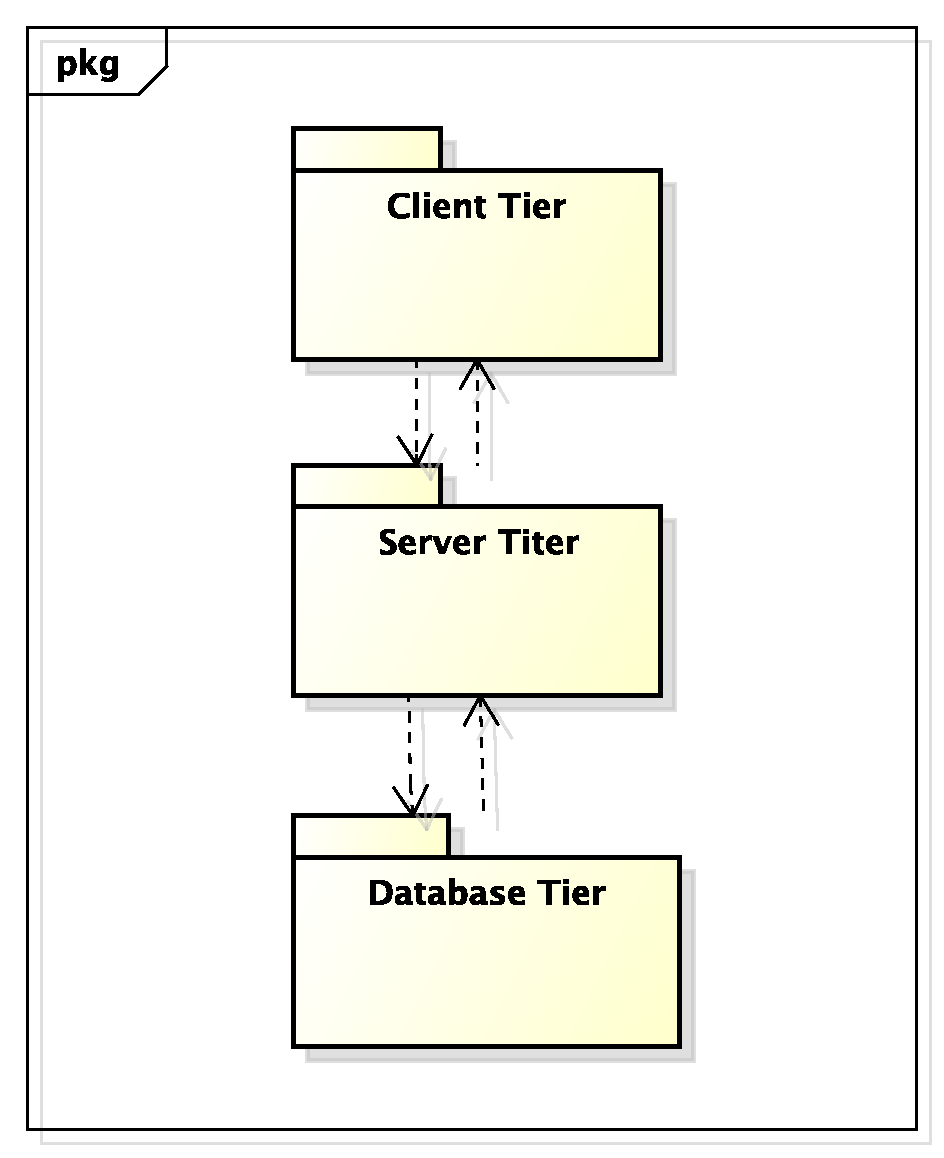
\includegraphics[scale=0.5]{./images/designpatternappendice/three_tier.pdf}}
			\caption{Design pattern architetturale - Three-Tier}
		\end{figure}


		\begin{itemize}
			\item \textbf{Scopo}: L'architettura Three-Tier, detta anche ``a tre strati'', identifica una particolare architettura software per l'esecuzione di un'applicazione web che prevede la suddivisione dell'applicazione in tre diversi moduli o strati dedicati rispettivamente all'interfaccia utente, alla logica funzionale e alla gestione dei dati persistenti. Tale architettura va tipicamente a mappare a livello fisico-infrastrutturale quella del sistema informatico ospitante l'applicazione da eseguire.
Tali moduli sono intesi interagire fra loro secondo le linee generali del paradigma client-server ( l'interfaccia è cliente della business logic, e questa è cliente del modulo di gestione dei dati persistenti) e utilizzando interfacce ben definite. In questo modo, ciascuno dei tre moduli può essere modificato o sostituito indipendentemente dagli altri conferendo scalabilità e manutenibilità all'applicazione. Nella maggior parte dei casi, i diversi moduli possono essere distribuiti su diversi nodi di una rete anche eterogenea;

			\item \textbf{Motivazione}: \'E stato scelto questo pattern perché il suo utilizzo è particolarmente diffuso nelle web application per poter disporre di moduli distribuiti, posti su piattaforme separate. Questa separazione aumenta le prestazioni e la scalabilità, l'estensibilità dei moduli e lo sviluppo parallelo degli stessi;

			\item \textbf{Applicabilità}: Oltre ai vantaggi abituali nell'utilizzare software modulare con interfacce ben definite, l'architettura Three-Tier consente anche a qualsiasi dei tre livelli di essere aggiornato o sostituito indipendentemente dal cambiamento di requisiti o tecnologia nell'applicazione;

		\end{itemize}
		% subsubsection three_tier (end)


		\newpage
		\subsubsection{MVC} % (fold)
		\begin{figure}[htbp]
			\centering
			\centerline{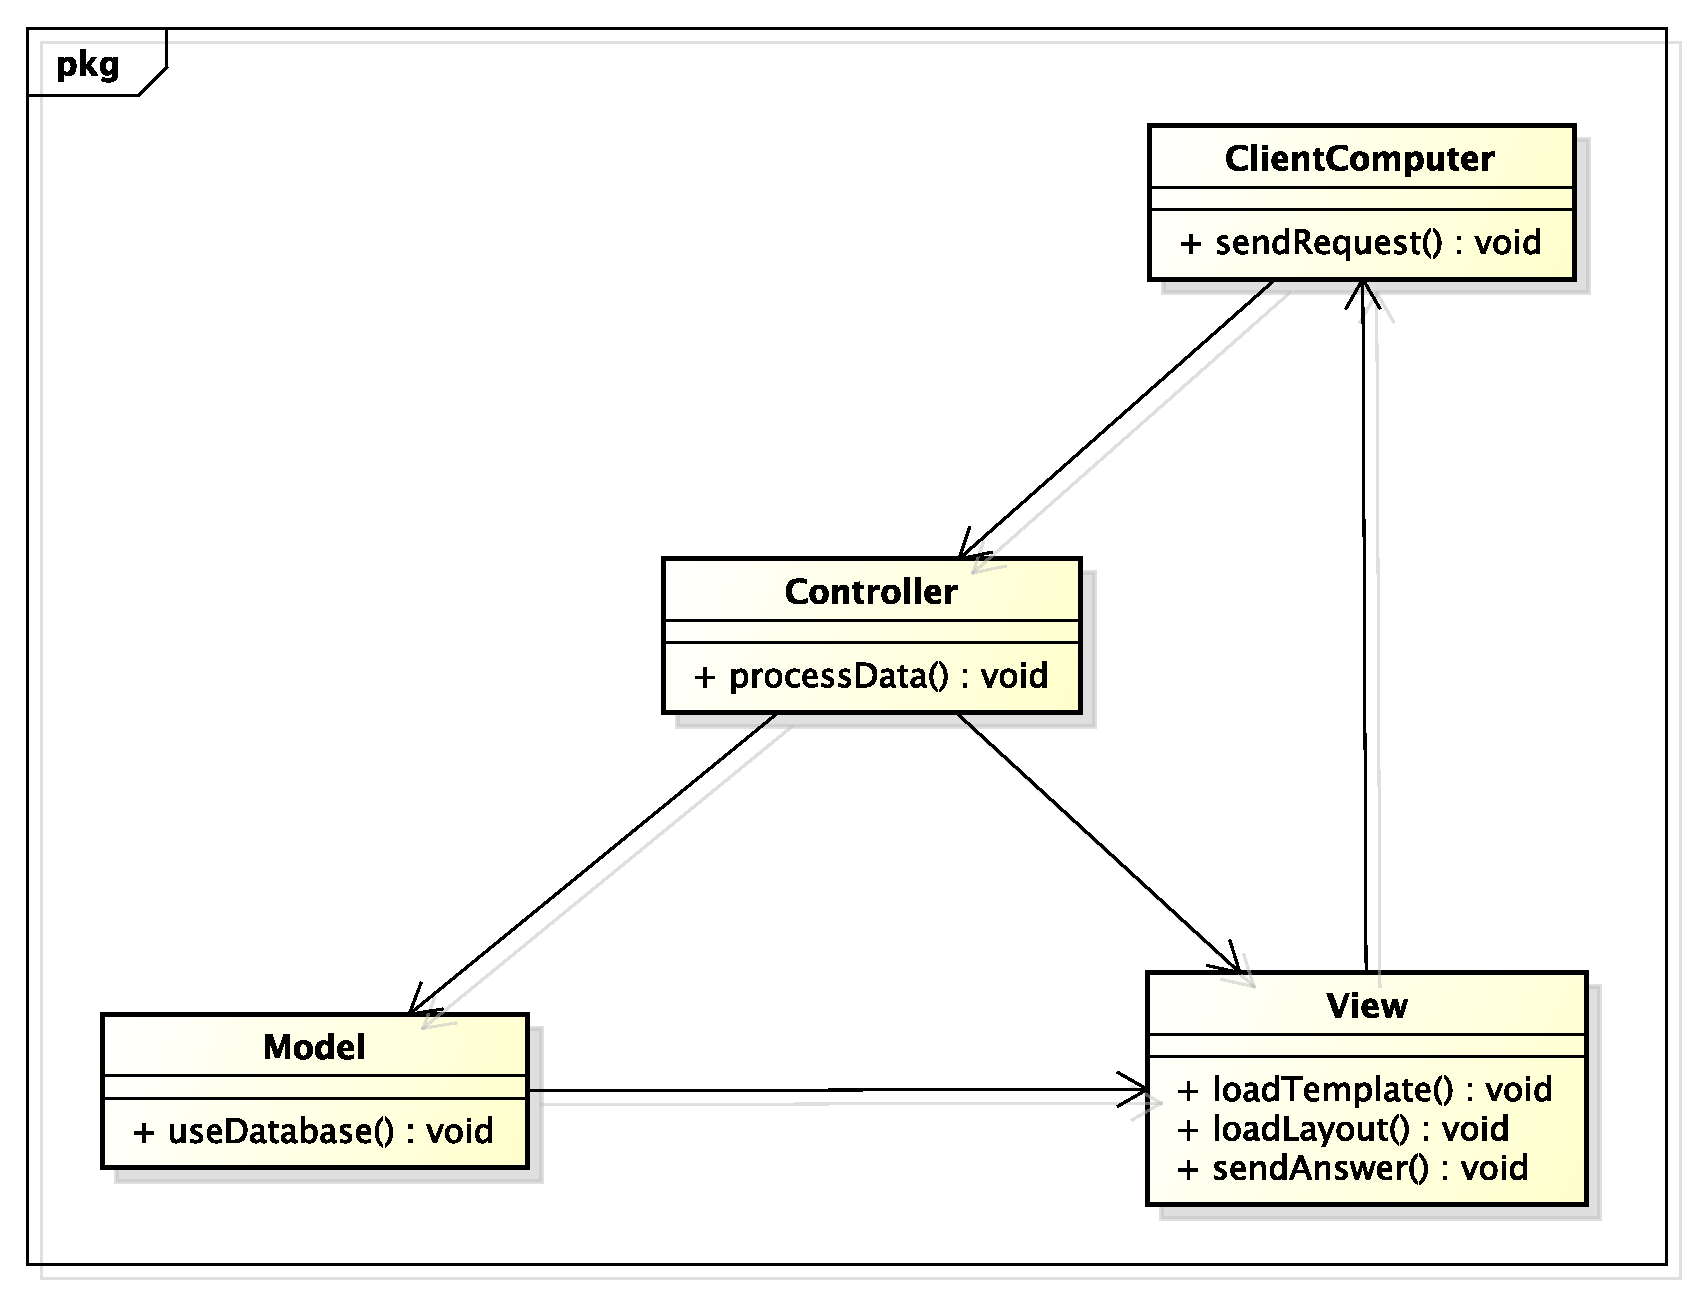
\includegraphics[scale=0.5]{./images/designpatternappendice/mvc.pdf}}
			\caption{Design pattern architetturale - MVC}
		\end{figure}

		\begin{itemize}
			\item \textbf{Scopo}: Il pattern è basato sulla separazione dei compiti fra i componenti software che interpretano tre ruoli principali:

		\begin{itemize}
			\item \textbf{Model} che fornisce i metodi per accedere ai dati utili all'applicazione;
			\item \textbf{View} che visualizza i dati contenuti nel model e si occupa dell'interazione con utenti e agenti;
			\item \textbf{Controller} che riceve i comandi dell'utente (in genere attraverso il view) e li attua modificando lo stato degli altri due componenti.
		\end{itemize}

		\noindent
		Questo schema implica anche la tradizionale separazione fra la logica applicativa (in questo contesto spesso chiamata ``logica di business''), a carico del Controller e del model, e l'interfaccia utente a carico del view. I dettagli delle interazioni fra questi tre oggetti software dipendono molto dalle tecnologie usate (linguaggio di programmazione, eventuali librerie, middleware e via dicendo) e dal tipo di applicazione (per esempio se si tratta di un'applicazione web, o di un'applicazione desktop). Quasi sempre la relazione fra view e model è descrivibile anche come istanza del pattern Observer. A volte, quando è necessario cambiare il comportamento standard dell'applicazione a seconda delle circostanze, il Controller implementa anche il pattern Strategy.;

			\item \textbf{Motivazione}: \'E stato scelto questo pattern perché è nata la necessità di rendere modulari le funzionalità dell'interfaccia utente. Utilizzando MVC viene quindi separata la modellazione dal dominio, dalla presentazione e dalle azioni basate sugli input degli utenti in tre classi separate;

			\item \textbf{Applicabilità}: Il pattern MVC può essere utilizzato in diversi casi:

			\begin{itemize}
			\item  Quando si vuole disaccoppiare View e Model instaurando un protocollo di sottoscrizione e notifica tra loro;
			\item Quando si vuole trattare un gruppo di oggetti come un oggetto singolo;
			\item Quando si vogliono agganciare più View a un Model per fornire più rappresentazioni del Model stesso;
			\end{itemize}

		\end{itemize}


		\newpage
		\subsubsection{MVVM} % (fold)
		\begin{figure}[htbp]
			\centering
			\centerline{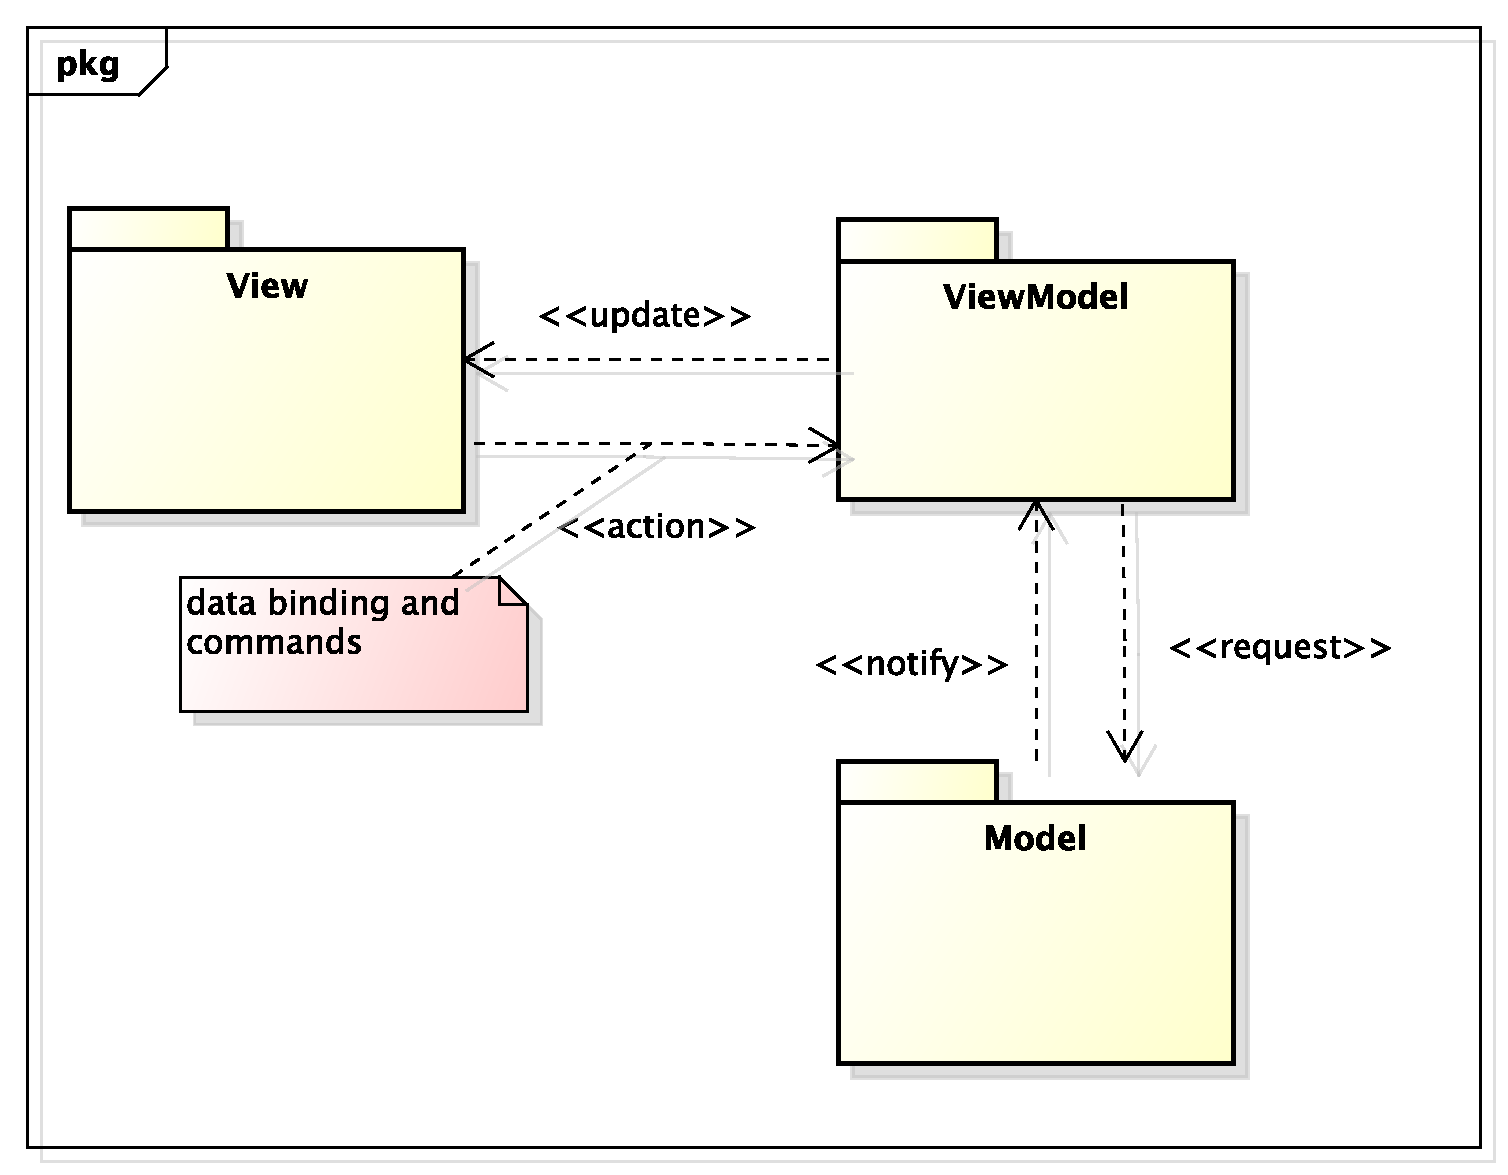
\includegraphics[scale=0.5]{./images/designpatternappendice/mvvm.pdf}}
			\caption{Design pattern architetturale - MVVM}
		\end{figure}

		\begin{itemize}
			\item \textbf{Scopo}: \'E una variante del pattern MVC. Questo pattern propone un ruolo più attivo della View rispetto a MVC: la View è in grado di gestire eventi, eseguire operazioni ed effettuare il data-binding. In questo contesto, quindi, alcune delle funzionalità del Controller vengono inglobate nella View, la quale si appoggia su un'estensione del Model: il ViewModel.
Il ViewModel è quindi un Model esteso con funzionalità per la manipolazione dei dati e per l'interazione con la View;

			\item \textbf{Motivazione}: \'E stato scelto questo pattern perché ha un impatto positivo nella progettazione di interfacce utente e viene implementato in modo semplice da Angular JS;

			\item \textbf{Applicabilità}: Il pattern MVVM è consigliato qualora si voglia separare interamente la progettazione dell'interfaccia grafica dalla business logic dell'applicazione;

		\end{itemize}

		\newpage
		\subsubsection{Dependency Injection} % (fold)

		\begin{figure}[htbp]
			\centering
			\centerline{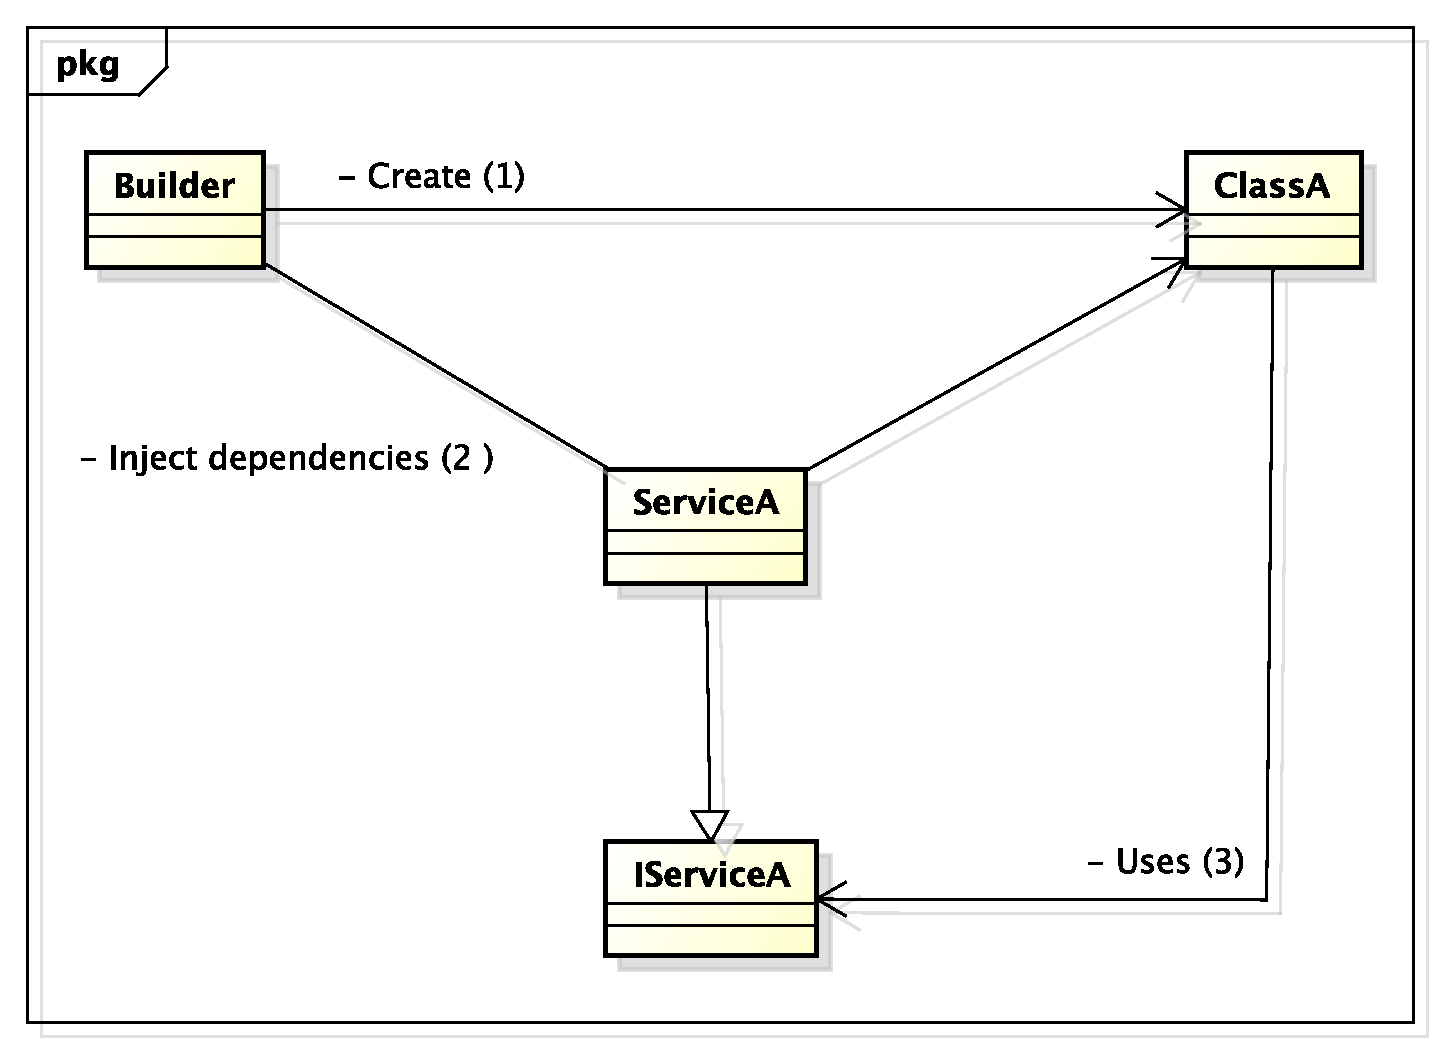
\includegraphics[scale=0.5]{./images/designpatternappendice/dep_injection.pdf}}
			\caption{Design pattern architetturale - Dependency Injection}
		\end{figure}

		\begin{itemize}
			\item \textbf{Scopo}: \'E quello di semplificare lo sviluppo e migliorare la testabilità di software di grandi dimensioni.
Il pattern Dependency Injection coinvolge almeno tre elementi:

				\begin{itemize}
					\item una componente dipendente;
					\item la dichiarazione delle dipendenze del componente, definite come interface contracts;
					\item un injector (chiamato anche provider o container) che crea, a richiesta, le istanze delle classi che implementano delle dependency interfaces;
				\end{itemize}

			\item \textbf{Motivazione}: \'E stato scelto questo pattern perché semplifica lo sviluppo e migliorare la testabilità di software di grandi dimensioni;

			\item \textbf{Applicabilità}: Il pattern Dependency Injection viene utilizzato principalmente nei seguenti casi di:
			\begin{itemize}
			\item Constructor Injection, dove la dipendenza viene iniettata tramite l’argomento del costruttore;
			\item Setter Injection, dove la dipendenza viene iniettata attraverso un metodo “set”;
			\item Interface Injection, che si basa sul mapping tra interfaccia e relativa implementazione;
			\end{itemize}
La Dependency Injection può essere realizzata in molteplici modi, tra cui il più semplice consiste nell'utilizzo di un factory method;

		\end{itemize}

	% subsection design_pattern_architetturali (end)


	\clearpage
	\newpage
	\subsection{Design pattern creazionali} % (fold)
		\subsubsection{Prototype Pattern} % (fold)

		\begin{figure}[htbp]
			\centering
			\centerline{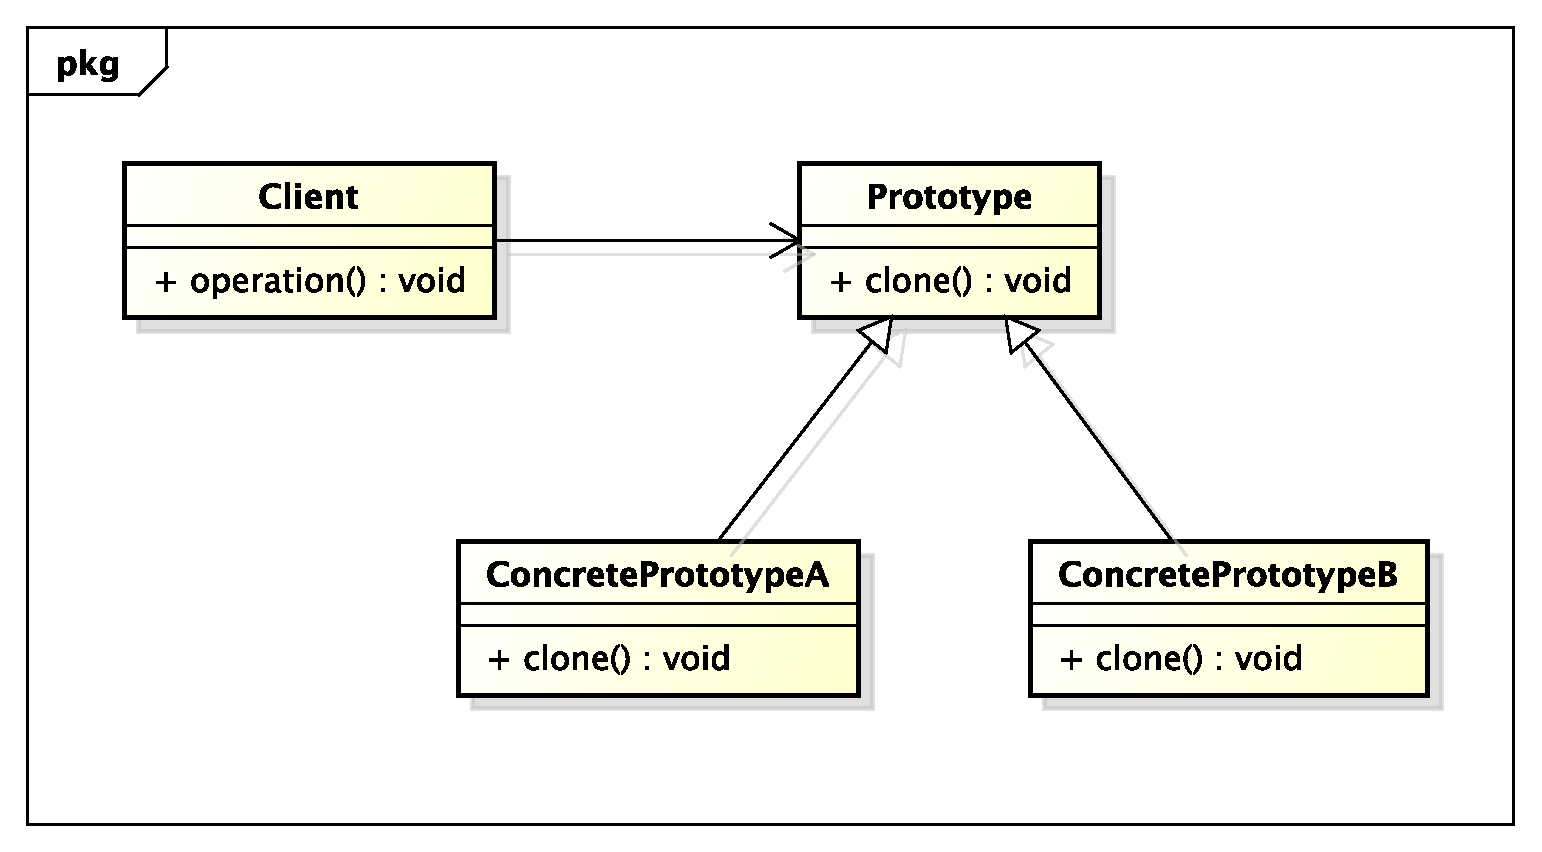
\includegraphics[scale=0.5]{./images/designpatternappendice/prototype.pdf}}
			\caption{Design pattern creazionale - Prototype Pattern}
		\end{figure}

		\begin{itemize}
			\item \textbf{Scopo}: Prototype permette di creare nuovi oggetti clonando un oggetto iniziale, detto appunto prototipo. A differenza di altri pattern come Abstract Factory o Factory Method permette di specificare nuovi oggetti a tempo d'esecuzione (run-time), utilizzando un gestore di prototipi ( detto prototype manager ) per salvare e reperire dinamicamente le istanze degli oggetti desiderati;

			\item \textbf{Motivazione}: \'E stato scelto questo pattern perché permette di incapsulare al suo interno la modalità di istanziazione degli oggetti, liberando il client dalla necessità di conoscere i nomi delle classi da istanziare. Inoltre permette di ridurre la complessità della gerarchia delle sottoclassi rispetto al Factory Method ed evitare la duplicazione di codice quando si usano diverse classi simili tra loro;

			\item \textbf{Applicabilità}: Come altri pattern creazionali, Prototype mira a rendere indipendente un sistema dal modo in cui i suoi oggetti vengono creati;

		\end{itemize}
		% subsubsection prototype_pattern (end)

		\newpage
		\subsubsection{Module Pattern} % (fold)
		\begin{figure}[htbp]
			\centering
			\centerline{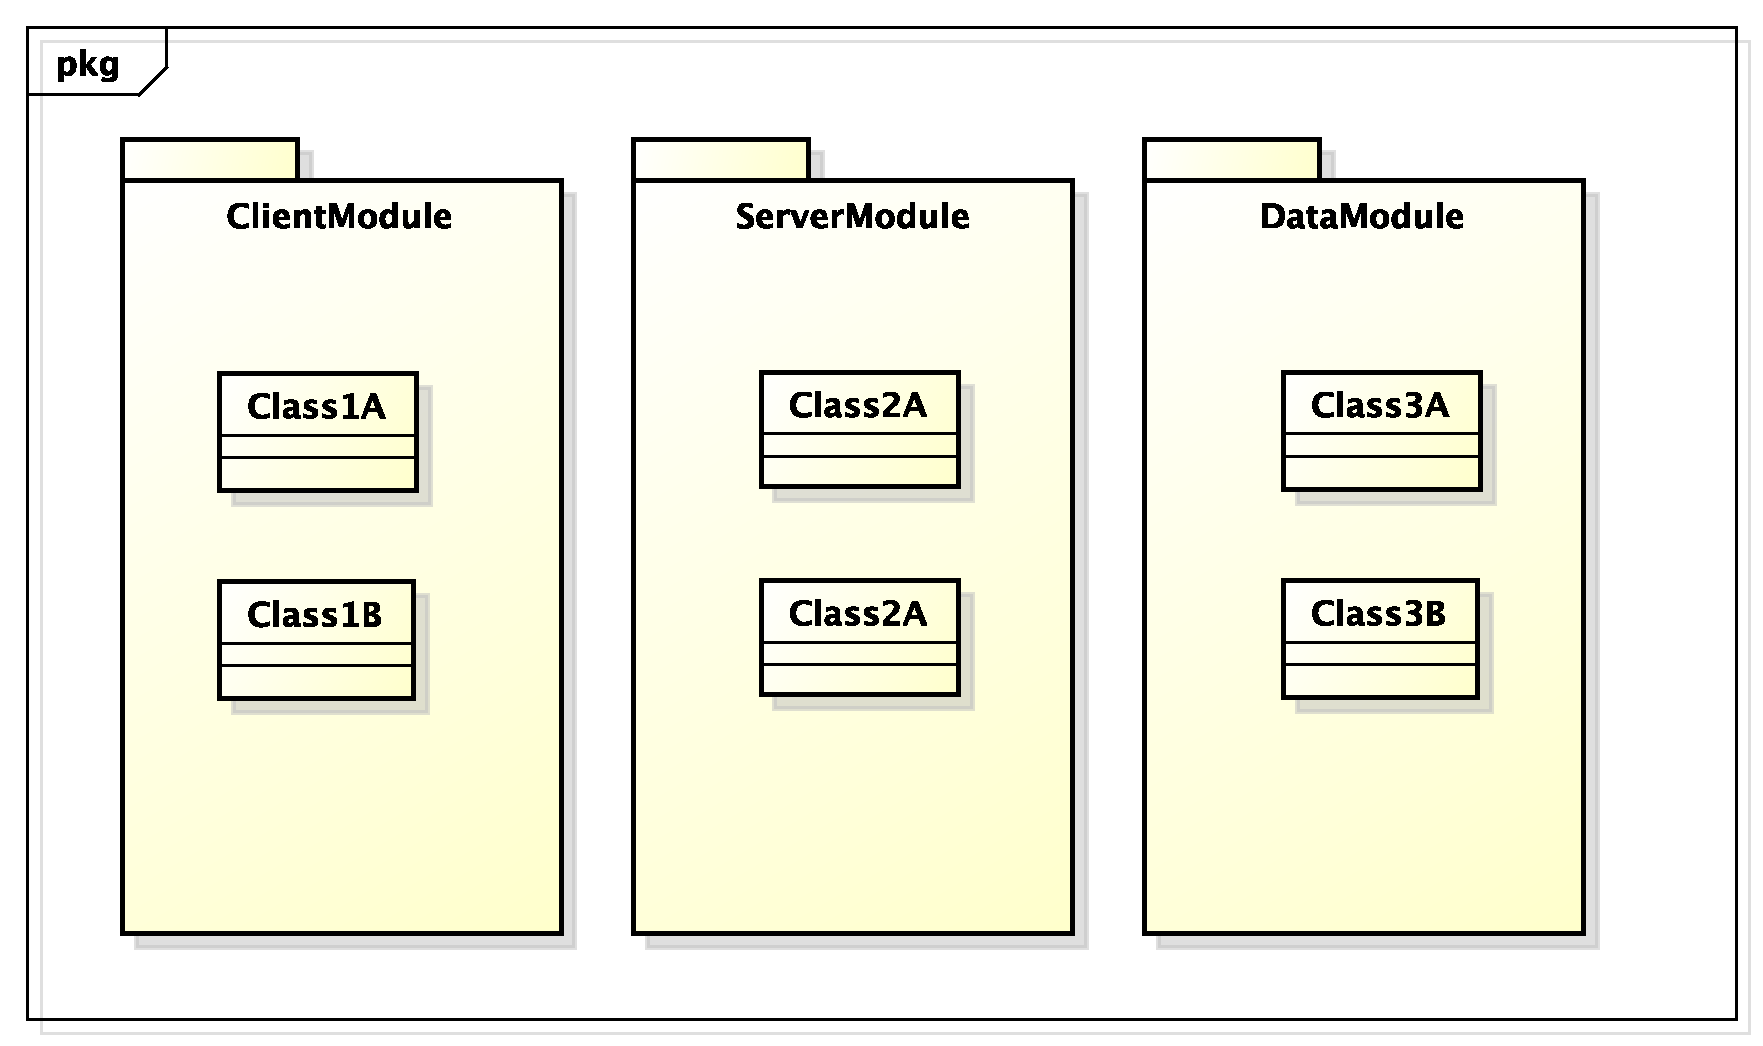
\includegraphics[scale=0.5]{./images/designpatternappendice/module_pattern.pdf}}
			\caption{Design pattern creazionale - Module Pattern}
		\end{figure}

		\begin{itemize}
			\item \textbf{Scopo}: Il module pattern prevede che l'applicazione che lo implementa sia divisa in moduli funzionali distinti. Essi consentono di organizzare le parti di un’applicazione in unità separate ma integrabili grazie ai meccanismi di esportazione e importazione, cioè rispettivamente della possibilità di rendere pubblicamente accessibile del codice e di accedere a codice esportato da altri moduli;

			\item \textbf{Motivazione}: \'E stato scelto questo pattern perché permette all'applicazione di essere robusta e facilmente manutenibile definendo un codice più chiaro e modulare. Permette inoltre una rapida risoluzione dei nomi, evitando ambiguità con i metodi e le variabili di altre funzioni globali;

			\item \textbf{Applicabilità}: Il module pattern è un design pattern usato per implementare il concetto dei moduli software in linguaggi di programmazione che non la supportano nativamente, come per esempio JavaScript;

		\end{itemize}
		% subsubsection module_pattern (end)

		\newpage
		\subsubsection{Singleton} % (fold)

		\begin{figure}[htbp]
			\centering
			\centerline{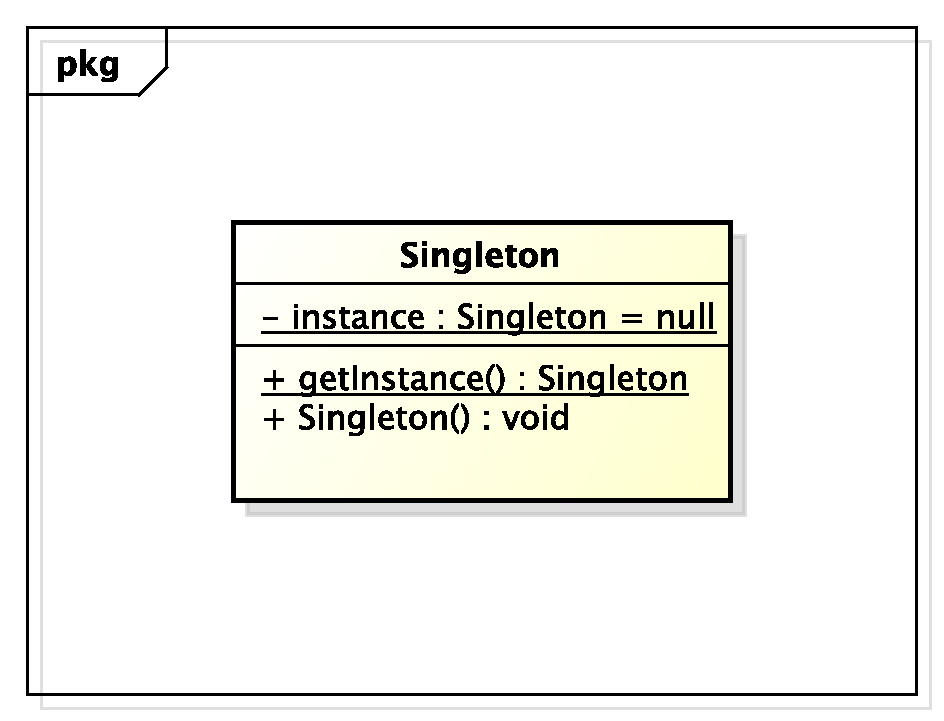
\includegraphics[scale=0.5]{./images/designpatternappendice/singleton.pdf}}
			\caption{Design pattern creazionale - Singleton}
		\end{figure}

		\begin{itemize}
			\item \textbf{Scopo}: Il singleton ha lo scopo di garantire che di una determinata classe venga creata una e una sola istanza, e di fornire un punto di accesso globale a tale istanza;

			\item \textbf{Motivazione}: \'E stato scelto questo pattern perché permette di creare istanze uniche di classi all'interno dell'applicazione;

			\item \textbf{Applicabilità}: Il pattern Singleton può essere utilizzato quando deve esistere una sola istanza di una classe in tutta l'applicazione e quando l'unica istanza deve poter essere estesa attraverso la definizione di sottoclassi garantendo che i client possano utilizzare le istanze estese senza dover modificare il proprio codice;
		\end{itemize}
		% subsubsection singleton (end)


	% subsection design_pattern_creazionali (end)


	\clearpage
	\newpage
	\subsection{Design pattern strutturali} % (fold)
		\subsubsection{Fa\c{c}ade} % (fold)
		\begin{figure}[htbp]
			\centering
			\centerline{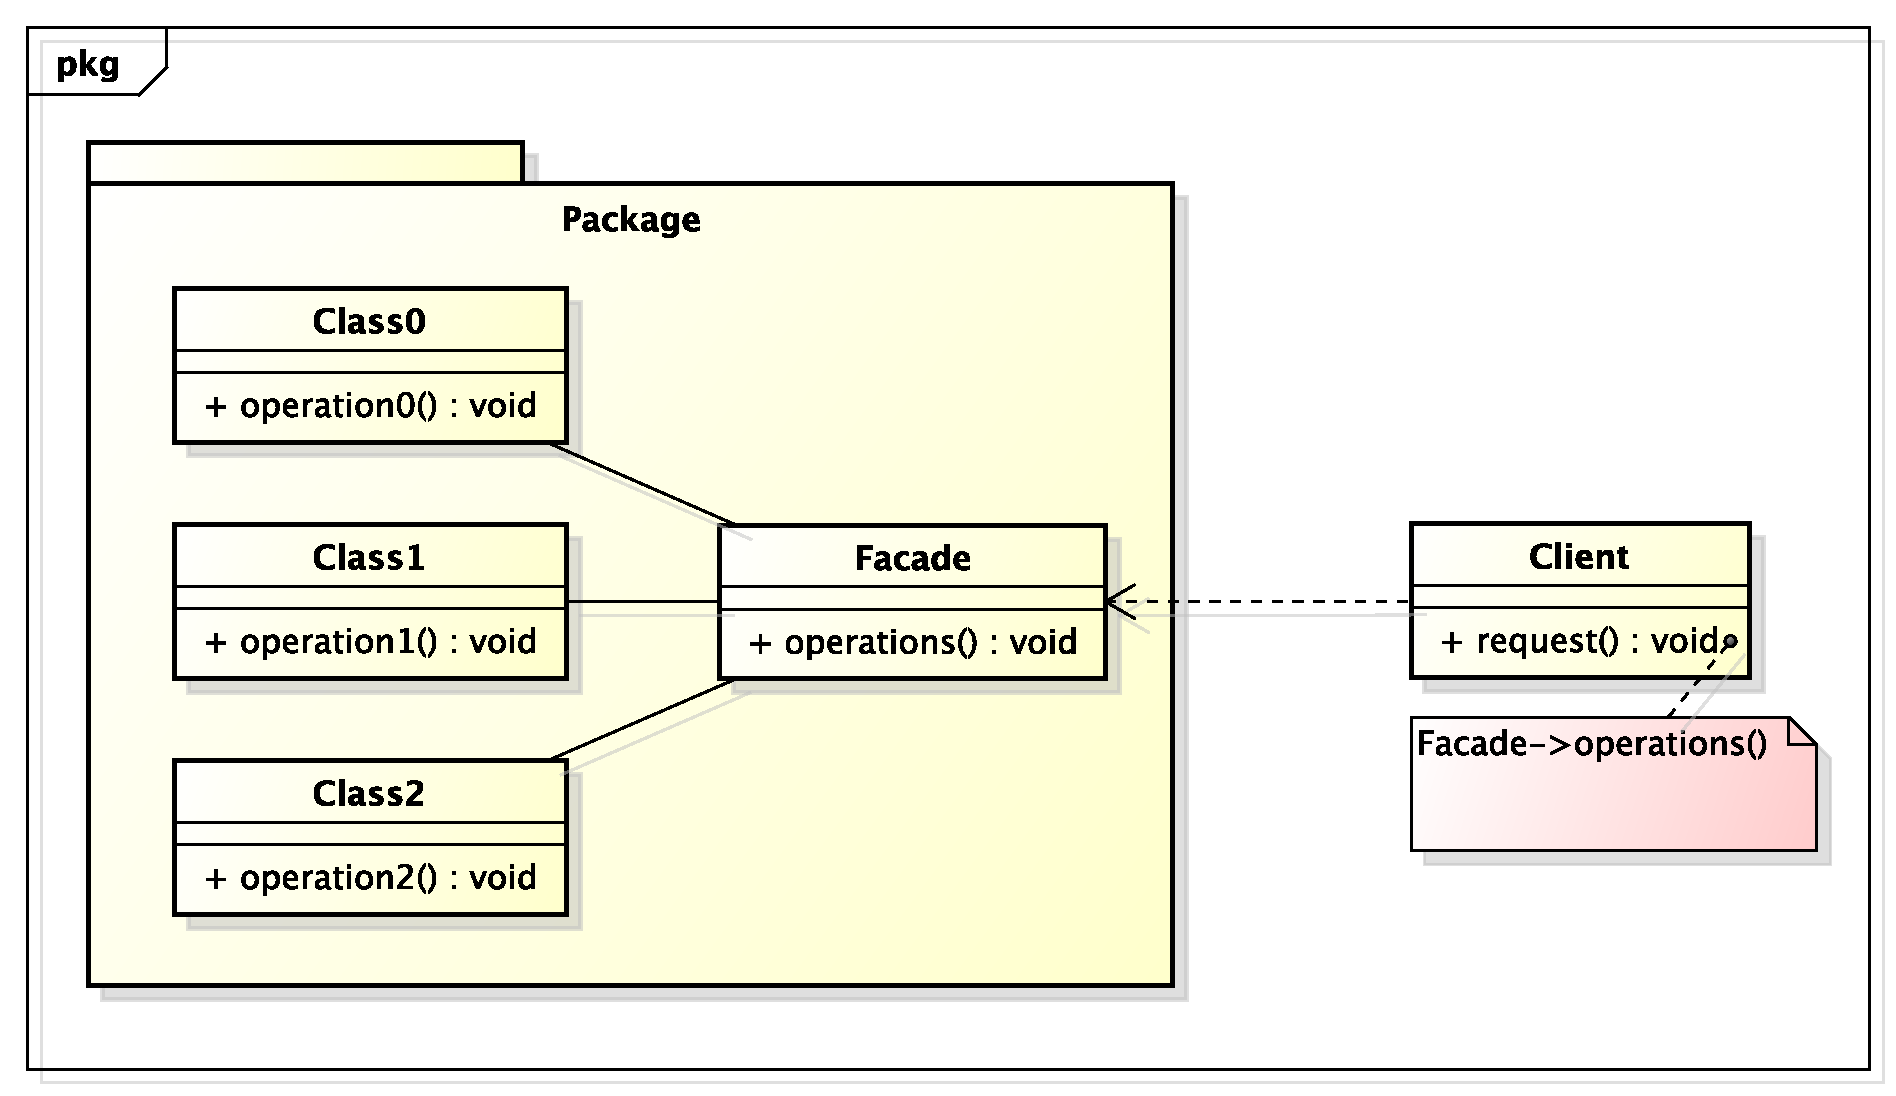
\includegraphics[scale=0.5]{./images/designpatternappendice/facade.pdf}}
			\caption{Design pattern strutturale - Fa\c{c}ade}
		\end{figure}

		\begin{itemize}
			\item \textbf{Scopo}: Il Fa\c{c}ade pattern suggerisce la creazione di un oggetto che presenti un'interfaccia semplificata al cliente, ma in grado di gestire tutta la complessità delle interazioni tra gli oggetti delle diverse classi per compiere l'obbiettivo desiderato;
			\item \textbf{Motivazione}: \'E stato scelto questo pattern perché fornisce una interfaccia unificata per un insieme di interfacce di un sottosistema, rendendo più facile l'uso di quest'ultimo;
			\item \textbf{Applicabilità}: Questo pattern può essere utilizzato per fornire una vista semplice e di default di un sottosistema complesso e nel caso di sottosistema stratificato, come entry point per ciascun livello;
		\end{itemize}



		\newpage
		\subsubsection{Adapter} % (fold)

		\begin{figure}[htbp]
			\centering
			\centerline{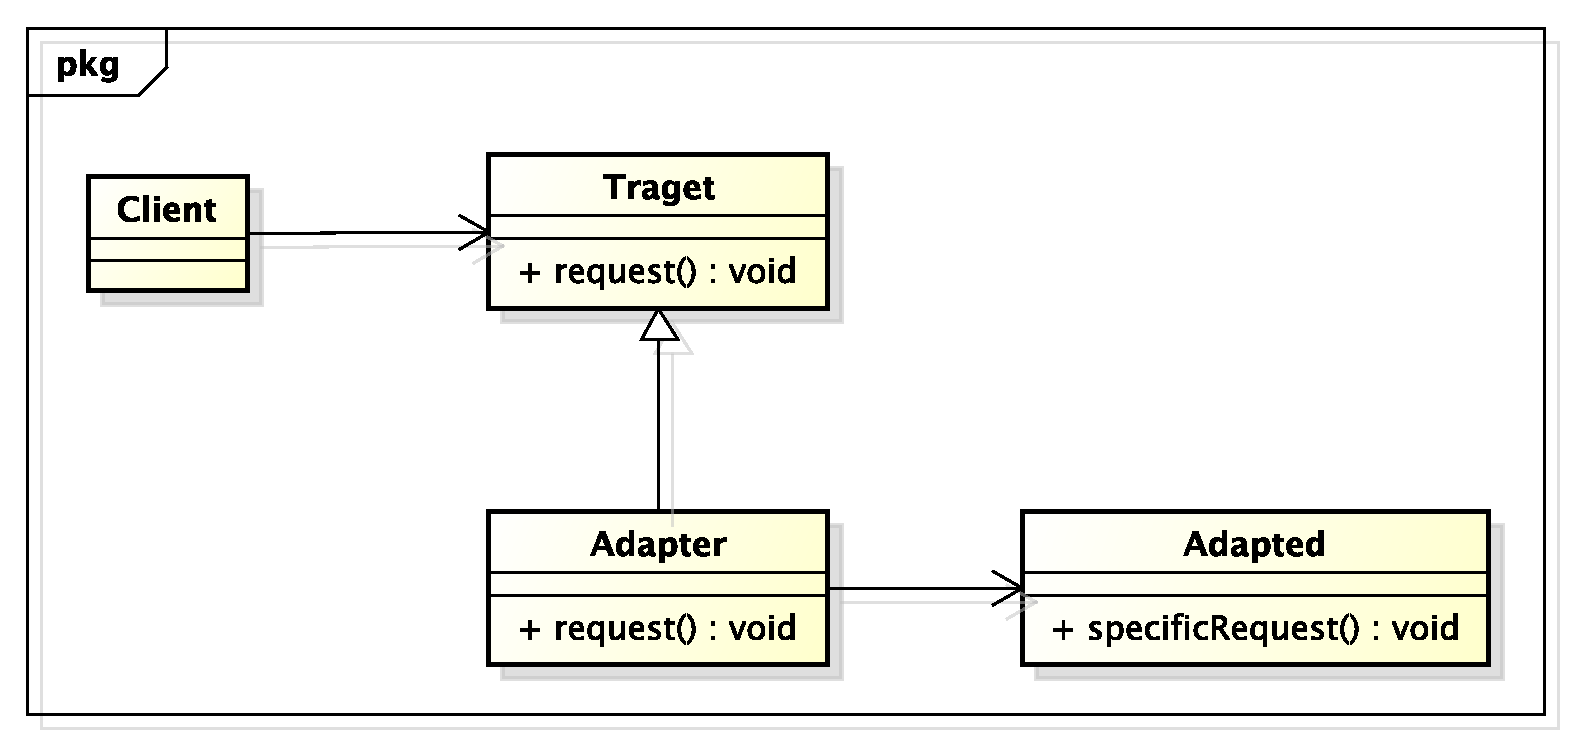
\includegraphics[scale=0.5]{./images/designpatternappendice/adapter.pdf}}
			\caption{Design pattern strutturale - Adapter}
		\end{figure}

		\begin{itemize}
			\item \textbf{Scopo}: Lo scopo è quello di fornire una soluzione astratta al problema dell'interoperabilità tra interfacce differenti. Questo problema si presenta ogni qual volta nel progetto di un software si debbano utilizzare oggetti la cui interfaccia non è perfettamente compatibile con quanto richiesto da applicazioni già esistenti. Invece di riscrivere parte del sistema, compito oneroso e non sempre possibile se non si ha a disposizione il codice sorgente, può essere comodo scrivere un adapter, appunto, che faccia da tramite;

			\item \textbf{Motivazione}: \'E stato scelto questo pattern perché permette l'interoperabilità tra diversi moduli, anche di terze parti, senza doverli modificare o riscrivere;

			\item \textbf{Applicabilità}: Questo pattern può essere utilizzato quando interfacce di classi differenti devono comunque poter comunicare tra loro. Alcuni casi sono:
			\begin{itemize}
			\item l'utilizzo di una classe esistente che presenti un'interfaccia diversa da quella desiderata;
			\item la scrittura di una determinata classe senza poter conoscere a priori le altre classi con cui dovrà operare;
			\end{itemize}

		\end{itemize}


	% subsection design_pattern_strutturali (end)

	\clearpage 
	\newpage
	\subsection{Design pattern comportamentali} % (fold)
		\subsubsection{Page Controller} % (fold)
		\begin{figure}[htbp]
			\centering
			\centerline{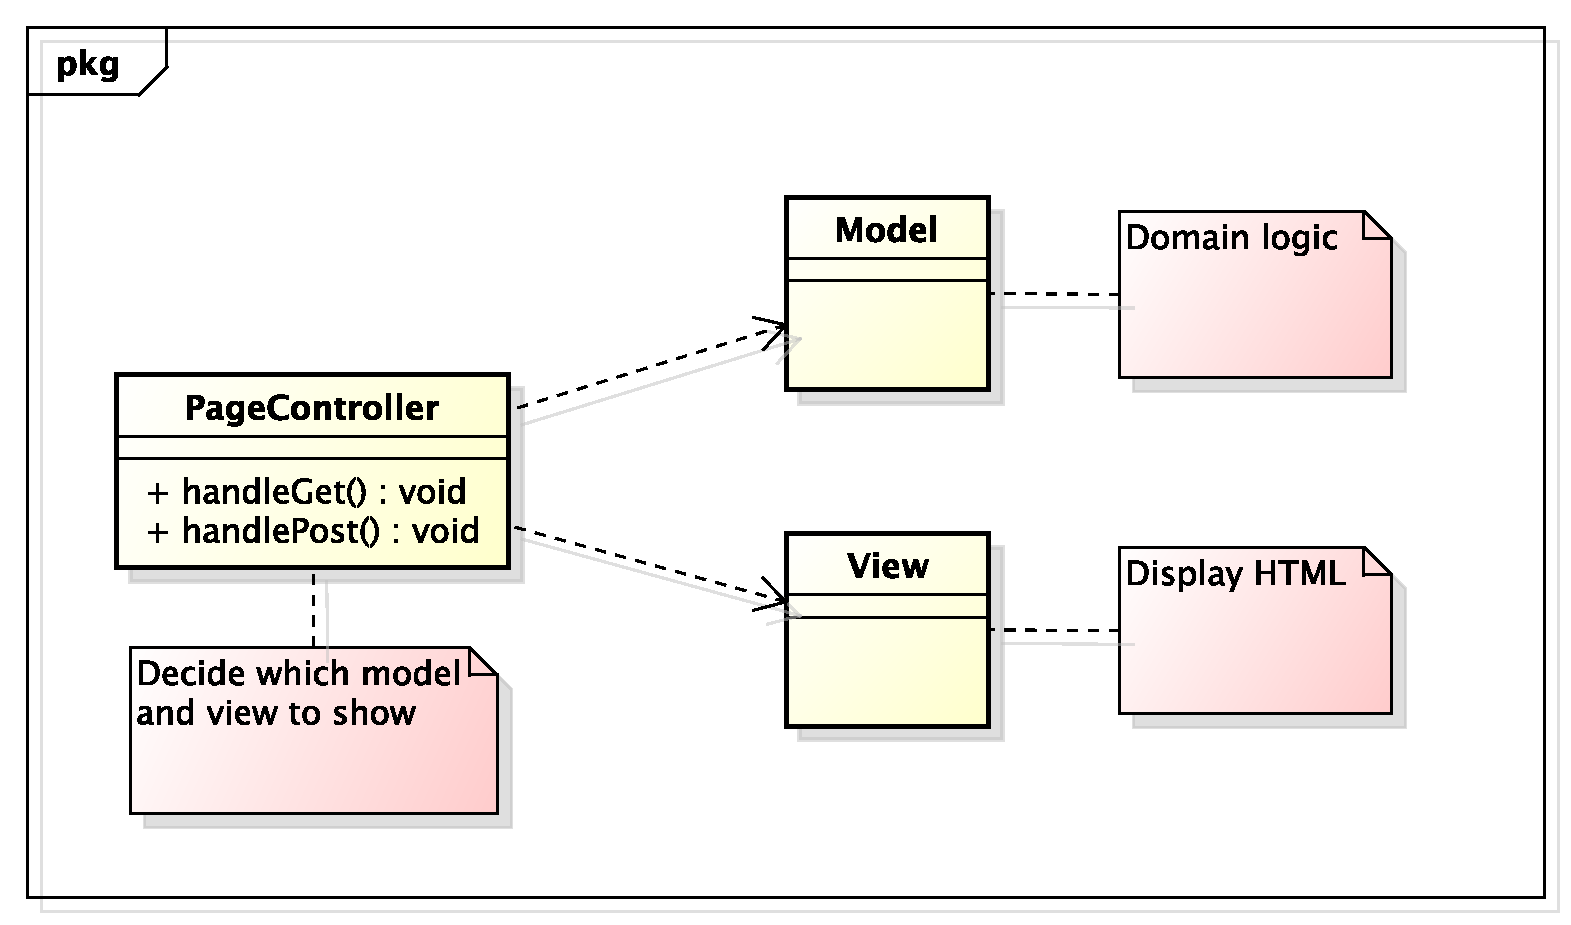
\includegraphics[scale=0.5]{./images/designpatternappendice/page_controller.pdf}}
			\caption{Design pattern comportamentale - Page Controller}
		\end{figure}

		\begin{itemize}
			\item \textbf{Scopo}: Il Page Controller pattern suggerisce la creazione di un oggetto dedicato che si occupa di gestire una richiesta per una specifica pagina o azione in un sito Web. Implica quindi che esiste un singolo file che gestisce la richiesta di una specifica pagina. Questo semplice meccanismo rispecchia il funzionamento delle pagine web statiche;
			\item \textbf{Motivazione}: \'E stato scelto questo pattern perché semplifica la gestione delle pagine web statiche utilizzate dall'applicazione e permette di eseguire test e riutilizzare codice in modo agevole;
			\item \textbf{Applicabilità}: Questo pattern può essere utilizzato in quei casi in cui si voglia utilizzare un singolo oggetto per gestire tutte le richieste di una singola pagina logica, a differenza del Front Controller che invece gestisce le richieste di molteplici pagine logiche con un singolo oggetto;
		\end{itemize}
		% subsubsection page_controller (end)

		\newpage
		\subsubsection{Template View} % (fold)
		\begin{figure}[htbp]
			\centering
			\centerline{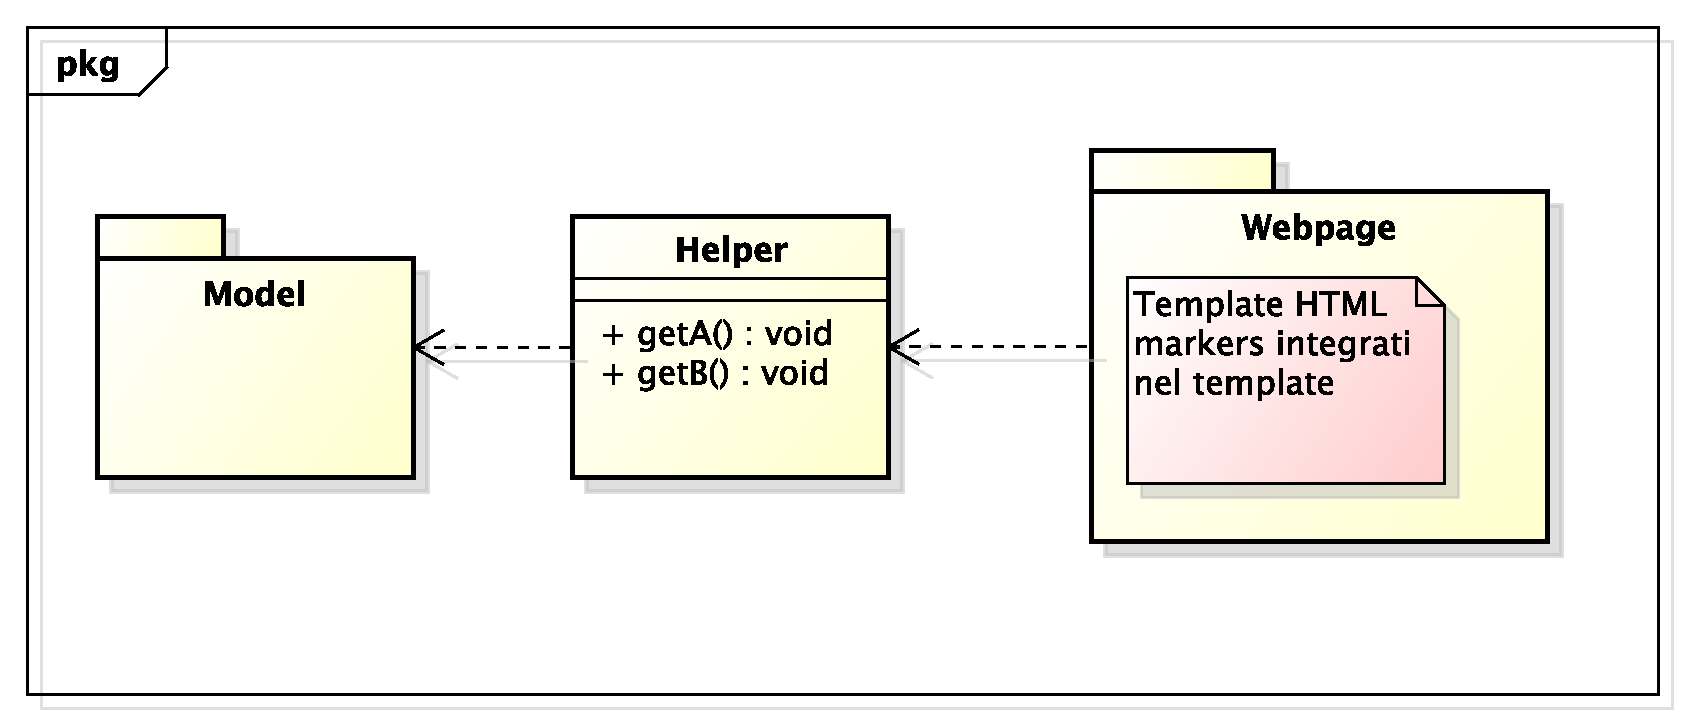
\includegraphics[scale=0.5]{./images/designpatternappendice/template_view.pdf}}
			\caption{Design pattern comportamentale - Template View}
		\end{figure}

		\begin{itemize}
			\item \textbf{Scopo}: Lo scopo di questo pattern è quello di implementare la componente View del design pattern Model View Controller mediante l'uso di template HTML. In questo modo i template svolgono il compito di isolare la presentation logic dal codice del linguaggio di programmazione utilizzato nell'applicazione web.
			\item \textbf{Motivazione}: \'E stato scelto questo pattern perché riduce in modo marcato la complessità della realizzazione di una pagina dinamica, tramite l'inserimento di marcatori in una struttura prefissata che serviranno come punti di ingresso per il contenuto dinamico generato;
			\item \textbf{Applicabilità}: Questo pattern viene utilizzato quando si vuole generare una pagina web dinamica allo stesso modo di una pagina web statica, definendo una struttura fissa e completandola con il contenuto dinamico richiesto;
		\end{itemize}
		% subsubsection template_view (end)

		\newpage
		\subsubsection{Template Method} % (fold)
		\label{ssub:template_method}
		\begin{figure}[htbp]
			\centering
			\centerline{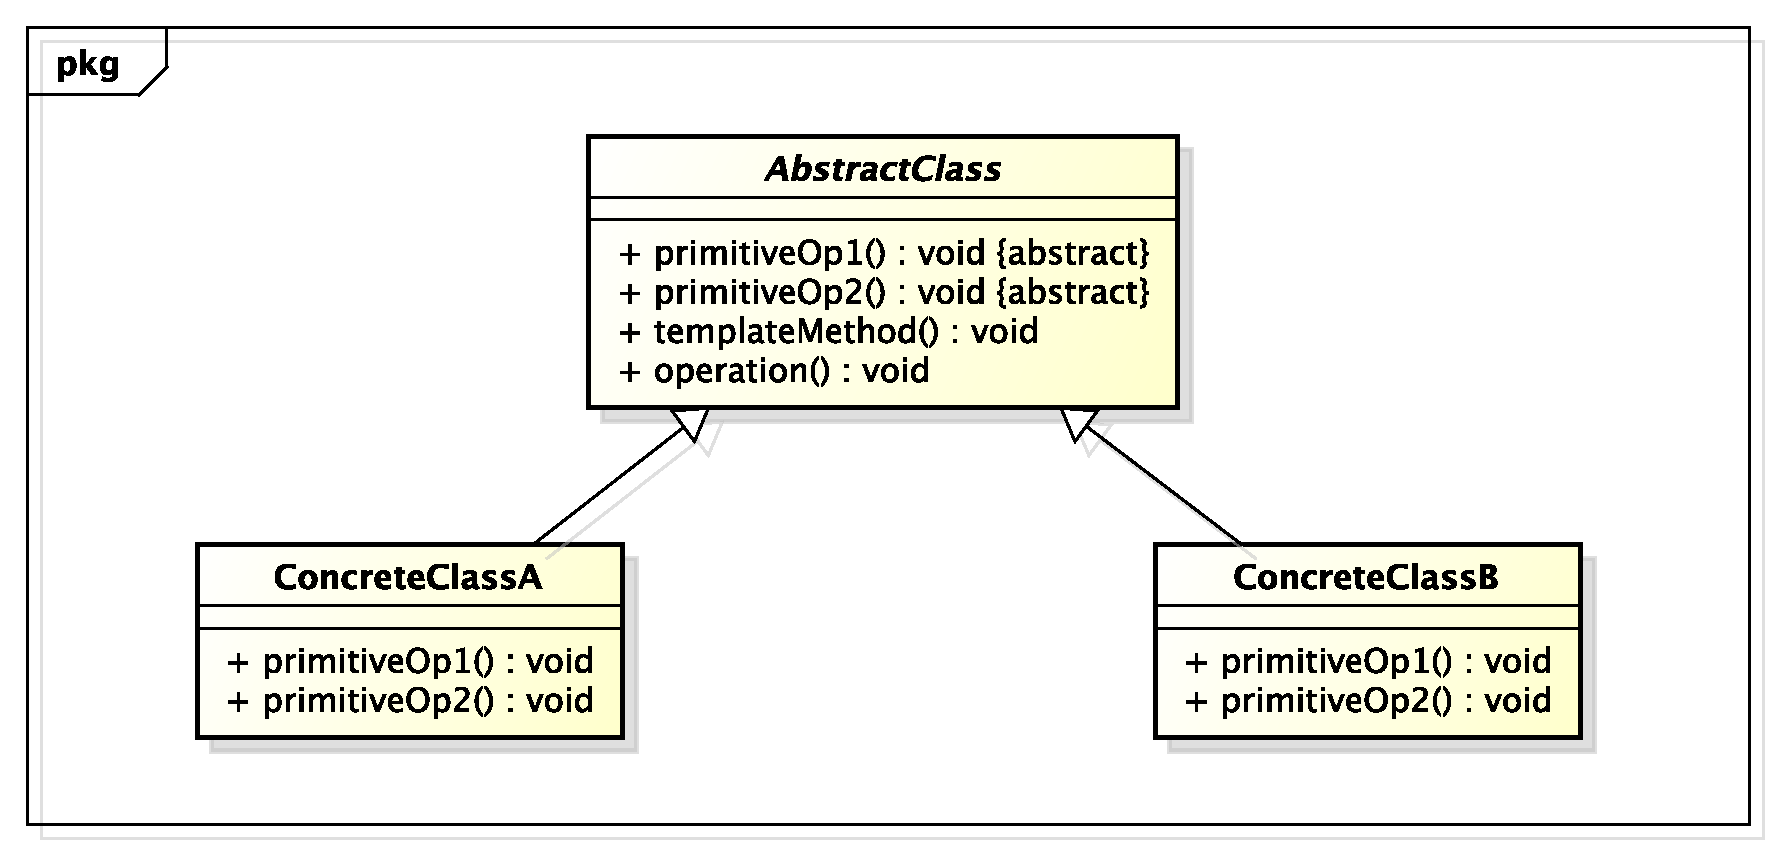
\includegraphics[scale=0.5]{./images/designpatternappendice/template_method.pdf}}
			\caption{Design pattern comportamentale - Template Method}
		\end{figure}
		\begin{itemize}
			\item \textbf{Scopo}: Il Template Method è un pattern comportamentale basato sulle classi e viene utilizzato prevalentemente nell'ambito della programmazione ad oggetti.
Questo pattern permette di definire la struttura di un algoritmo delegando alle sottoclassi il compito di implementarne alcuni passi. In questo modo si può ridefinire e personalizzare parte del comportamento nelle varie sottoclassi senza dover riscrivere più volte il codice in comune nella classe principale;
			\item \textbf{Motivazione}: \'E stato scelto questo pattern perché permette una maggior libertà nella definizione dei metodi, dando la possibilità di lavorare nelle sottoclassi senza dover apportare modifiche alla classe astratta principale;
			\item \textbf{Applicabilità}: Questo pattern può essere utilizzato nei seguenti casi:
			\begin{itemize}
			\item quando si vuole implementare la parte invariante di un algoritmo una volta sola e lasciare che le sottoclassi implementino il comportamento variabile dello stesso;
			\item quando il comportamento comune di più classi può essere inserito all'interno di una classe a parte per evitare la duplicazione di codice;
			\item per avere modo di controllare quali metodi vengono ereditati dalla super-classe, facendo in modo che i metodi template siano gli unici metodi sovra scrivibili;
			\end{itemize}

		\end{itemize}
		% subsubsection template_method (end)


		\newpage
		\subsubsection{Command} % (fold)
		\label{ssub:command}
		\begin{figure}[htbp]
			\centering
			\centerline{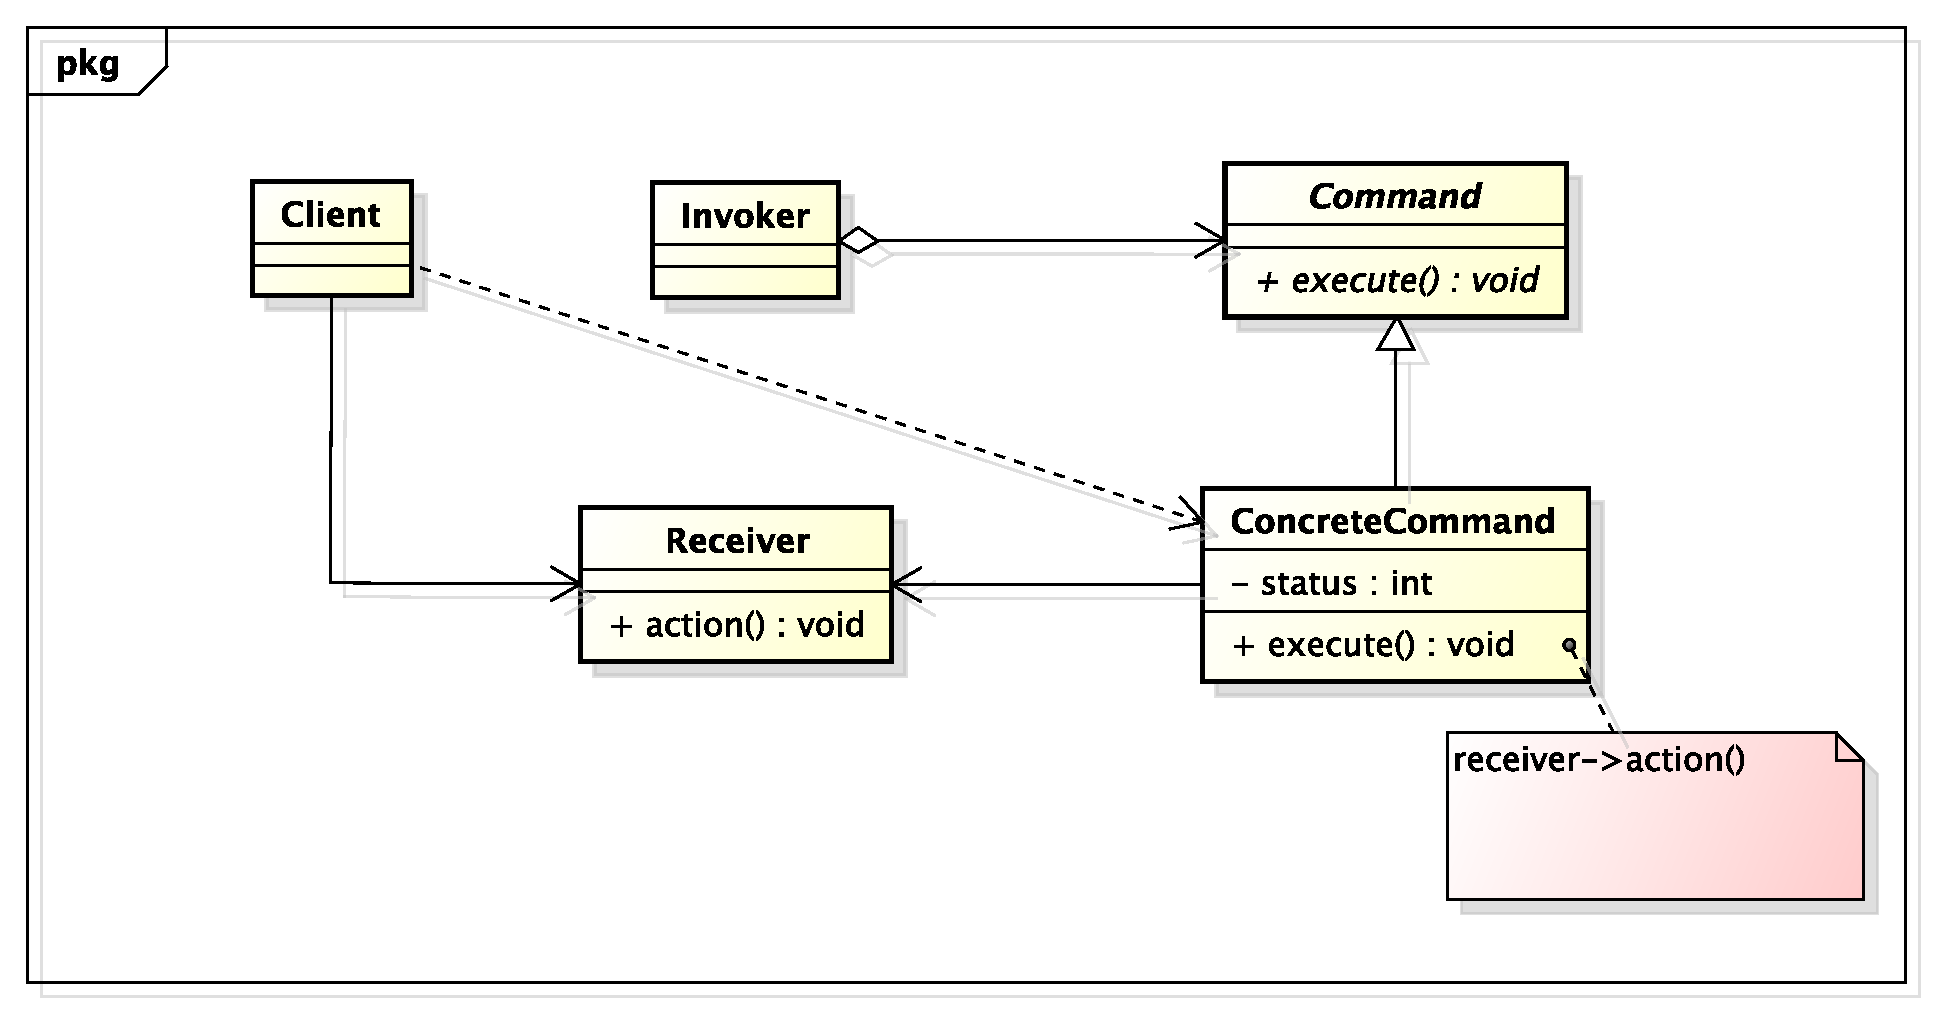
\includegraphics[scale=0.5]{./images/designpatternappendice/command.pdf}}
			\caption{Design pattern comportamentale - Command}
		\end{figure}
		
		\begin{itemize}
			\item \textbf{Scopo}: Il Command pattern permette di isolare la porzione di codice che effettua un'azione anche molto complessa dal codice che ne richiede l'esecuzione; l'azione viene tipicamente incapsulata in un oggetto specifico detto ``command''. 
			L'obiettivo è rendere variabile l'azione del client senza però conoscere i dettagli dell'operazione stessa. Un altro aspetto importante è che il destinatario della richiesta può non essere deciso staticamente all'atto dell'istanziazione dell'oggetto ``command'' ma ricavato a tempo di esecuzione;
			\item \textbf{Motivazione}: \'E stato scelto questo pattern perché permette agli oggetti ``command'' di essere decisi dinamicamente in base all'operazione che bisogna eseguire;
			\item \textbf{Applicabilità}: Questo pattern può essere utilizzato nei casi in cui:
			\begin{itemize}
			\item si richiede che un'azione sia atomica: si può implementare un oggetto di comando in modo che le transazioni al suo interno vengano svolte in toto o per nulla;
			\item si vuole rendere asincrona la scelta dei comandi rispetto alla loro esecuzione. Un certo numero di ``command'' possono essere elaborati da un altro oggetto che li riceve in un tempo diverso dalla loro selezione;
			\end{itemize}

		\end{itemize}
		% subsubsection command (end)

	% subsection design_pattern_comportamentali (end)


% section descdp (end)